\documentclass{article}

\usepackage{graphicx}
\usepackage{tikz-cd}
\usepackage[margin=0.25in]{geometry}

\begin{document}

\begin{center}
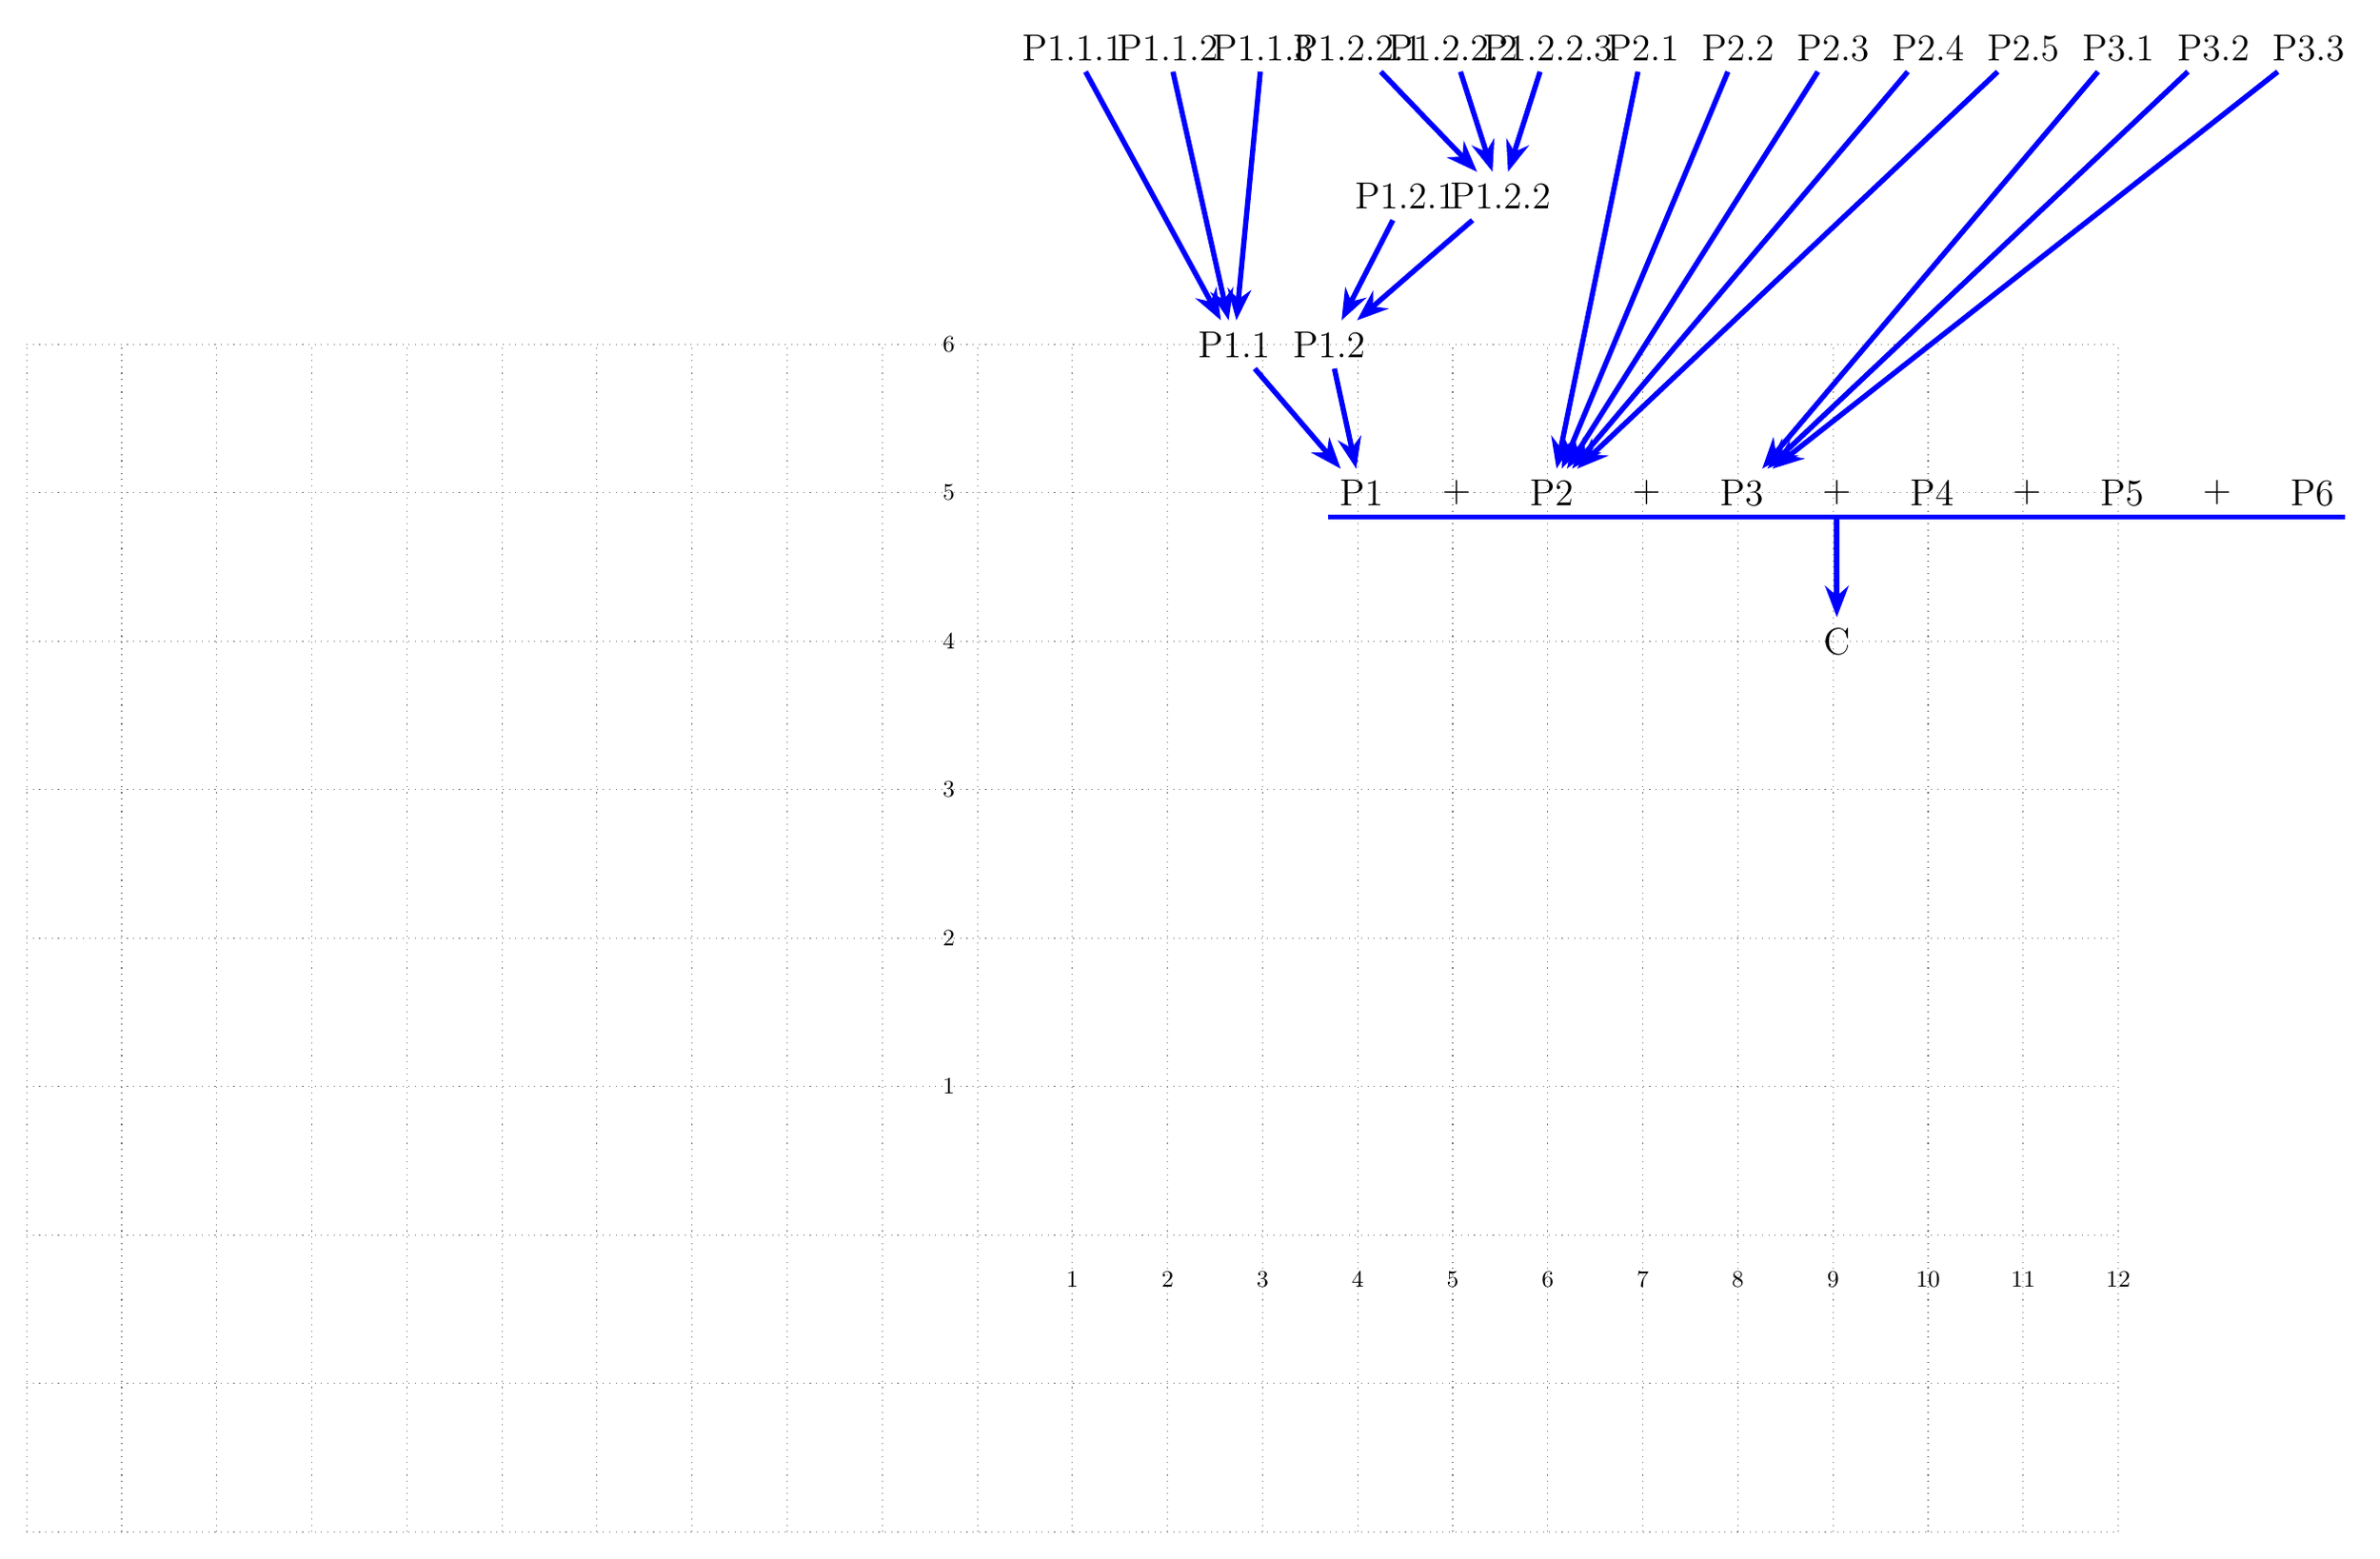
\begin{tikzpicture}[
	>=Stealth, 
	line width=2pt, 
	x=1.28cm,y=2.0cm, 
	font=\fontsize{14}{14}\selectfont
	]
	% begin grid
\draw[step=1, gray, thin, dotted] (-10,-2) grid (12,6);

% Grid numbers
\foreach \x in {1,2,3,4,5,6,7,8,9,10,11,12}
\node at (\x, -0.3) {\small \x};
\foreach \y in {1,2,3,4,5,6}
\node at (-0.3, \y) {\small \y};

% end grid
 

			\node (p1_2_2_1_4_8)   at (4.0, 8) {P1.2.2.1};
			\node (p1_2_2_2_5_8)   at (5.0, 8) {P1.2.2.2};
			\node (p1_2_2_3_6_8)   at (6.0, 8) {P1.2.2.3};
			\node (p1_1_1_1_8)   at (1.0, 8) {P1.1.1};
			\node (p1_1_2_2_8)   at (2.0, 8) {P1.1.2};
			\node (p1_1_3_3_8)   at (3.0, 8) {P1.1.3};
			\node (p2_1_7_8)   at (7.0, 8) {P2.1};
			\node (p2_2_8_8)   at (8.0, 8) {P2.2};
			\node (p2_3_9_8)   at (9.0, 8) {P2.3};
			\node (p2_4_10_8)   at (10.0, 8) {P2.4};
			\node (p2_5_11_8)   at (11.0, 8) {P2.5};
			\node (p3_1_12_8)   at (12.0, 8) {P3.1};
			\node (p3_2_13_8)   at (13.0, 8) {P3.2};
			\node (p3_3_14_8)   at (14.0, 8) {P3.3};
			\node (p1_2_1_4_7)   at (4.5, 7) {P1.2.1};
			\node (p1_2_2_5_7)   at (5.5, 7) {P1.2.2};
			\node (p1_1_2_6)   at (2.7, 6) {P1.1};
			\node (p1_2_3_6)   at (3.7, 6) {P1.2};
			\node (p1_4_5)   at (4.040000000000001, 5) {P1};
			\node (plus_5_5)   at (5.040000000000001, 5) {+};
			\node (p2_6_5)   at (6.040000000000001, 5) {P2};
			\node (plus_7_5)   at (7.040000000000001, 5) {+};
			\node (p3_8_5)   at (8.040000000000001, 5) {P3};
			\node (plus_9_5)   at (9.040000000000001, 5) {+};
			\node (p4_10_5)   at (10.040000000000001, 5) {P4};
			\node (plus_11_5)   at (11.040000000000001, 5) {+};
			\node (p5_12_5)   at (12.040000000000001, 5) {P5};
			\node (plus_13_5)   at (13.040000000000001, 5) {+};
			\node (p6_14_5)   at (14.040000000000001, 5) {P6};
			\node (c_9_4)   at (9.040000000000001, 4) {C};

			\draw[->, blue] (p1_2_2_1_4_8) -- (p1_2_2_5_7);
			\draw[->, blue] (p1_2_2_2_5_8) -- (p1_2_2_5_7);
			\draw[->, blue] (p1_2_2_3_6_8) -- (p1_2_2_5_7);
			\draw[->, blue] (p1_1_1_1_8) -- (p1_1_2_6);
			\draw[->, blue] (p1_1_2_2_8) -- (p1_1_2_6);
			\draw[->, blue] (p1_1_3_3_8) -- (p1_1_2_6);
			\draw[->, blue] (p1_2_1_4_7) -- (p1_2_3_6);
			\draw[->, blue] (p1_2_2_5_7) -- (p1_2_3_6);
			\draw[->, blue] (p1_1_2_6) -- (p1_4_5);
			\draw[->, blue] (p1_2_3_6) -- (p1_4_5);
			\draw[->, blue] (p2_1_7_8) -- (p2_6_5);
			\draw[->, blue] (p2_2_8_8) -- (p2_6_5);
			\draw[->, blue] (p2_3_9_8) -- (p2_6_5);
			\draw[->, blue] (p2_4_10_8) -- (p2_6_5);
			\draw[->, blue] (p2_5_11_8) -- (p2_6_5);
			\draw[->, blue] (p3_1_12_8) -- (p3_8_5);
			\draw[->, blue] (p3_2_13_8) -- (p3_8_5);
			\draw[->, blue] (p3_3_14_8) -- (p3_8_5);
			\draw[->, blue] (plus_9_5) -- (c_9_4);

			\draw[blue] (p1_4_5.south west) -- (p6_14_5.south east);

\end{tikzpicture}

\section{test}

Some text

\end{center}

\end{document}
